\chapter{Particle in a Central Potential. The Hydrogen Atom}\footnote{Cohen}
In thsi chapter, we shall consider the quantum mechanical properties of a particle placed in a central potential [that is, a potential $V(r)$ which depends only on the distance $r$ from the origin]. This problem is closely related to the study of angular momentum. As we shall know, the fact that $V(r)$ es invariant under any rotation about the origin means that the Hamiltonian $H$ of the particle conmutes with the three components of the orbital angular momentum operator $\vb{L}$. This cosiderably simplifies the determination of the eigenfunctions and eigenvalues of $\vb{L}^2$ and $L_z$ as well.



\section{Statioanary states of a particle in a central potential}
In this section, we consider a (spinless) particle of mass $\mu$, subjected to a central force derived from the potential $V(r)$ (the center of force is chosen as the origin).
\subsection{Outline of the problem}
\subsubsection{Review of some classical results}
The force acring on the classical particle situated at the point $M$ (with $\vb{OM}=\vb{r}$) is equal to:
\begin{equation}\label{A-1}
	\vb{F}=-\nabla V(r)=-\dv{V}{r}\frac{\vb{r}}{r}
\end{equation}
$\vb{F}$ is always directed towards $O$,  and its mimentum with respect to this point is therefore always zero. If:
\begin{equation}\label{A-2}
	\vb{\mathcal{L}}=\vb{r}\times\vb{p}
\end{equation}
is the angular momentum of the particle with respecto to $O$, the anfular momentum theorem implies that:
\begin{equation}\label{A-3}
	\dv{\vb{\mathcal{L}}}{t}=\vb{0}
\end{equation}
$\vb{\mathcal{L}}$ is therefore a \textit{constant of the motion}, so that the particle's trajectory is necessarily situated in the plane passing through $O$ and perpendicular to $\vb{\mathcal{L}}$.

\begin{figure}[h]
	\begin{center}
		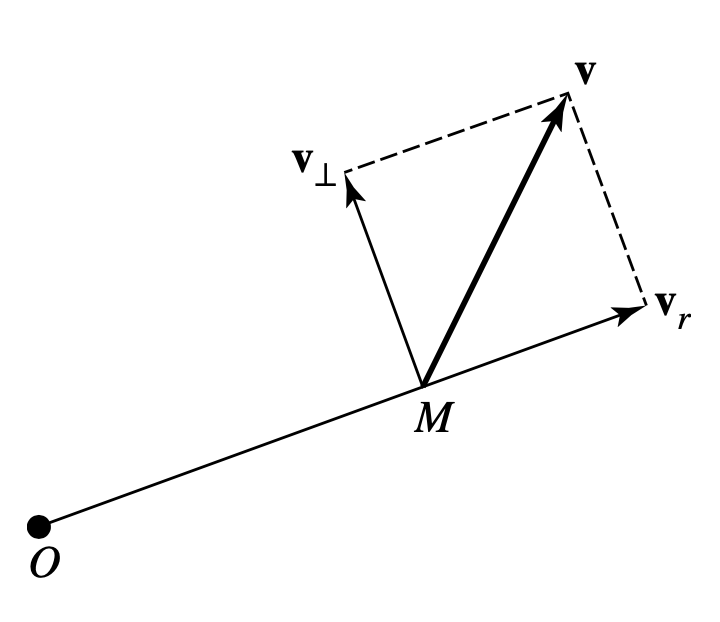
\includegraphics[scale=0.6]{fig/fig1-A-cohen.png}
		\caption{Radial component $\vb{v}_r$ and tangential component $\vb{v}_\perp$ of a particle's velocity.}
		\label{fig:1-a-cohen}
	\end{center}	
\end{figure}

Now let us consider Fig. \ref{fig:1-a-cohen} the position (denoted by $\vb{OM}=\vb{r}$) and velocity $\vb{v}$ of the particle at the instant $t$. Thw two vectors $\vb{r}$ and $\vb{v}$ lie in the plane of the trajectory and the velocity $\vb{v}$ can be decomposed into the radial component $\vb{v}_r$ (along the axis defined by $\vb{r}$) and the tangential component $\vb{v}_\perp$ (along the axis perpendicular to $\vb{r}$). The radual velocity, the algebraic value of $\vb{v}_r$, is the time derivative of the distance of the particle from the point $O$:
\begin{equation}\label{A-4}
	v_r=\dv{r}{t}
\end{equation}
The tangential velociry can be expressed in term of $r$ and the angular momentum $\vb{\mathcal{L}}$, since:
\begin{equation}\label{A-5}
	|\vb{r}\times\vb{v}|=r|\vb{v}_\perp|
\end{equation}
so that the modulus of the angular momentum $\vb{\mathcal{L}}$ is equal to:
\begin{equation}\label{A-6}
	|\vb{\mathcal{L}}|=|\vb{r}\times\mu\vb{v}|=\mu r|\vb{v}_\perp|
\end{equation}
The total energy of the particle:
\begin{equation}\label{A-7}
	E=\frac{1}{2}\mu\vb{v}^2+V(r)=\frac{1}{2}\mu \vb{v}_r^2+\frac{1}{2}\mu \vb{v}_\perp^2+V(r)
\end{equation}
can be written:
\begin{equation}\label{A-8}
	E=\frac{1}{2}\mu\vb{v}_r^2+\frac{\vb{\mathcal{L}}^2}{2\mu r^2}+V(r)
\end{equation}
The classical Hamiltonian if the system is then:
\begin{equation}\label{A-9}
	\mathcal{H}=\frac{p_r^2}{2\mu}+\frac{\vb{\mathcal{L}}^2}{2\mu r^2} + V(r)
\end{equation}
where:
\begin{equation}\label{A-10}
	p_r=\mu\dv{r}{t}
\end{equation}
is the conjugate momentum of $r$,  and $\vb{\mathcal{L}}^2$ must be expressed in terms of the variables $r, \theta, \varphi$ and their conjugate momenta $p_r,p_\theta,p_\varphi$. One finds:
\begin{equation}\label{A-11}
	\vb{\mathcal{L}}^2=p_\theta ^2 +\frac{1}{\sin^2\theta}p_\varphi^2
\end{equation}
In expression (\ref{A-9}), the kinetic energy is broken into two terms: the radial kinetic energy and the kinetic energy of rotation about $O$ . The reason is that, since $V(r)$ is independent of $\theta$ and $\varphi$ in this case, the angular variables and their conjugate momenta appear only in the $\vb{\mathcal{L}}^2$ term. In fact, if we are interested in the evolution of $r$, we can use the fact that $\vb{\mathcal{L}}$ is a constant of the motion, and replace $\vb{\mathcal{L}}^2$ by a constant in expression (\ref{A-9}). The Hamiltonian $\mathcal{H}$  then appears as a function only of the radial variables $r$ and $p_r$ ( $\vb{\mathcal{L}}^2$ plays the role of a parameter), and the result is a differential equation involving only one variable, $r$:
\begin{equation}\label{A-12a}
	\dv{p_r}{t}=\mu\dv[2]{r}{t}=-\pdv{\mathcal{H}}{r}
\end{equation}
that is:
\begin{equation}\label{A-12b}
	\mu\pdv[2]{r}{t}=\frac{\vb{\mathcal{L}}^2}{\mu r^2}-\dv{V}{r}
\end{equation}
It is just as if we had a one-dimensional problem (with $r$ varyng only between $0$ and $+\infty$), with a particle of mass $\mu$ subjected to the "efective potential":
\begin{equation}\label{A-13}
	V_{eff}(r)=V(r)+\frac{\vb{\mathcal{L}}^2}{2\mu r^2}
\end{equation}
We shall see that the situation is analogous in quantum mechanics.


\subsubsection{The quantum mechanical Hamiltonian}
In quantum mechanics, we want to solve the eigenvalue equation of the Hamiltonian $\mathcal{H}$, the observable associated with the total energy. This equation is written, in the $\{\ket{\vb{r}}\}$ representation:
\begin{equation}\label{A-14}
	\left[-\frac{\hbar^2}{2\mu}\Delta +V(r)\right]\varphi(\vb{r}) = E\varphi(\vb{r})
\end{equation}
Since the potential $V$ depends only on the distance  $r $of the particle from the origin, spherical coordinates are best adapted to the problem. We therefore express the Laplacian $\Delta$ in spherical coordinates \footnote{Expression (\ref{A-15}) gives the Laplacian only for non-zero $r$. This is because of the privileged position of the origin in spherical coordinates; it can be seen, moreover, that expression (\ref{A-15}) is not defined for $r=0$.}
\begin{equation}\label{A-15}
	\Delta = \frac{1}{r}\pdv[2]{r}r+\frac{1}{r^2}\left(\pdv[2]{\theta} +\frac{1}{\tan\theta}\pdv{\theta}+\frac{1}{\sin^2\theta}\pdv[2]{\varphi}\right)
\end{equation}
and look for eigenfucntions $\varphi(\vb{r})$ that are functions of the variables $r,\theta,\varphi$.

If we compare expression (\ref{A-15}) with the one for the operator $\vb{\mathcal{L}}^2$, wee see that the quantum mechanical Hamiltonian $\mathcal{H}$ can be put in a form completely analogous to (\ref{A-9}):
\begin{equation}\label{A-16}
	\boxed{H=-\frac{\hbar^2}{2\mu}\frac{1}{r}\pdv[2]{r}+\frac{1}{2\mu r^2}\vb{L}^2+V(r)}
\end{equation}
The angular dependence of the Hamiltonian is contained entirely in the $\vb{L}^2$ term, which is an operator here. We could, in fact, perfect the analogy by defining an operator $P_r$, which would allow us to write the first term of (\ref{A-16}) like the one in (\ref{A-9}).

We shall now show how one can solve the eigenvalue equation:
\begin{equation}\label{A-17}
	\left[-\frac{\hbar^2}{2\mu}\frac{1}{r}\pdv[2]{r}+\frac{1}{2\mu r^2}\vb{L}^2+V(r)\right]\varphi(r,\theta,\varphi)=E\varphi(r,\theta,\varphi)
\end{equation}

\subsection{Separation of variables}
\subsubsection{Angular dependence of the eigenfunctions}
We know that the three components of the angular momentum operator $\vb{L}$ act only on the angular variables $\theta$ and $\varphi$ ; consequently, they commute with all operators acting only on the $r$-dependence. In addition, they commute with $\vb{L}^2$. Therefore, according to expression (\ref{A-16}) for the Hamiltonian, \textit{the three components of L are constants of the motion\footnote{(\ref{A-18}) express the fact that $H$ is a scalar operator with respect to rotations about the point $O$. This is true because the potential energy is invariant under rotations about $O$.}} in the quantum mechanical sense:
\begin{equation}\label{A-18}
	[H,\vb{L}]=\vb{0}
\end{equation}

Obviously, $H$ also commutes with $\vb{L}^2$.

Although we have at our disposition four constants of the motion ($L_x,L_y,L_z$ and $\vb{L}^2$), we cannot use all four of them to solve equation (\ref{A-17}) because they do not commute with each other; we shall use only $\vb{L}^2$ and $L_z$. Since the three observables $H$, $\vb{L}^2$ and $L_z$ commute, we can find a basis of the state space $\mathcal{E}_r$ of the particle composed of eigenfunctions common to these three observables. We can, therefore,  require the functions $\varphi(r,\theta,\varphi)$, solutions of equation (\ref{A-17}), to be eigenfunctions of $\vb{L}^2$ and $L_z$  as well. We must then solve the system of differential equations:
\begin{align}
	\label{A-19a}H\varphi(\vb{r})&=E\varphi(\vb{r})\\
	\label{A-19b}\vb{L}^2\varphi(\vb{r})&=l(l+1)\hbar^2\varphi(\vb{r})\\
	L_z\varphi(\vb{r})&=m\hbar \varphi(\vb{r}) \label{A-19c}
\end{align}
But we already know the general form of the common eigenfunctions of $\vb{L}^2$ and $L_z$: the solutions $\varphi(\vb{r})$ of equations (\ref{A-19a}), (\ref{A-19b}), (\ref{A-19c}) corresponding to fixed values $l$ of and $m$ , are necessarily products of a function of $r$ alone and the spherical harmonic $Y_l^m(\theta,\varphi)$:
\begin{equation}\label{A-20}
	\varphi(\vb{r})=R(r)Y_l^m(\theta,\varphi)
\end{equation}
Whatever the radial function $R(r)$, $\varphi(\vb{r})$ is a solution of equations (\ref{A-19b}) and (\ref{A-19c}). The only problem which remains to be solved is therefore how to determine $R(r)$ such that $\varphi(\vb{r})$ is also an eigenfunction of $H$ [equation (\ref{A-19a})].

\subsubsection{The radial equation}
We shall now substitute expressions (\ref{A-16}) and (\ref{A-20}) into (\ref{A-19a}). Since $\varphi(\vb{r})$ is an eigenfunction of $\vb{L}^2$ with the eigenvalue $l(l+1)\hbar^2$, we see that $Y_l^m(\theta,\varphi)$ is a common factor on both sides. After simplifyng, we obtain the radial equation:
\begin{equation}\label{A-21}
	\left[-\frac{\hbar^2}{2\mu}\frac{1}{r}\dv[2]{r}r+\frac{l(l+1)\hbar^2}{2\mu r^2}+V(r)\right]R(r)=ER(r)
\end{equation}
Actually, a solution of (\ref{A-21}), substituted into (\ref{A-20}), does not necessarily yield a solution of the eigenvalue equation (\ref{A-14}) of the Hamiltonian. As we have already pointed out, expression (\ref{A-15}) for the Laplacian is not necessarily valid at $r=0$. We must therefore make sure that the behavior of the solutions $R(r$) of (\ref{A-21}) at the origin is sufficiently regular for (\ref{A-20}) to be in fact a solution of (\ref{A-14}).

Instead of solving the partial differential equation (\ref{A-17}) involving the three variables $r,\theta\varphi$ we must now solve a differential equation involving only the variable $r$, but dependent on a parameter $l$: we are looking for eigenvalues and eigenfunctions of an operator $H_l$ which is different for each value of $l$.

In other words, we consider separately, in the state space $\mathcal{E}_r$, the subspaces $\mathcal{E}(l,m)$ corresponding to fixed values of $l$ and $m$ , studying the eigenvalue equation of $H$ in each of these subspaces (which is possible because $H$ commutes with $\vb{L}^2$ and $L_z$). The equation to be solved depends on $l$ , but not on $m$ ; it is therefore the same in the $(2l+1)$ subspaces $\mathcal{E}(l,m)$ associated with a given value of $l$. We shall denote by $_{k,l}$ the eigenvalues of $H_l$ , that is, the eigenvalues of the Hamiltonian $H$ inside a given subspace $\mathcal{E}(l,m)$. The index $k$, which can be discrete or continuous, represents the various eigenvalues associated with the same value of $l$. As for the eigenfunctions of $H_l$, we shall label them with the same two indices as the eigenvalues: $R_{k,l}(r)$. It is not obvious that this is sufficient: several radial functions might exist and be eigenfunctions of the same operator $H_l$ with the same eigenvalue $E_{k,l}$; we shall see that this is not the case and that, consequently, the two indices $k $and $l$ are sufficient to characterize the different radial functions. We shall therefore rewrite equation (\ref{A-21}) in the form:
\begin{equation}\label{A-22}
	\left[-\frac{\hbar^2}{2\mu}\frac{1}{r}\dv[2]{r}+\frac{l(l+1)\hbar^2}{2\mu r^2}+V(r)\right]R_{k,l}(r)=E_{k,l}R_{k,l}(r)
\end{equation}
We can simplify the differential operator to be studied by a change in functions.

We set:
\begin{equation}\label{A-23}
	R_{k,l}(r)=\frac{1}{r}u_{k,l}(r)
\end{equation}
Multiplying both sides of (\ref{A-22}) by $r$, we obtain for $u_{k,l}(r)$ the following differential equation:
\begin{equation}\label{A-24}
	\boxed{\left[-\frac{\hbar^2}{2\mu}\dv[2]{r}+\frac{l(l+1)\hbar^2}{2\mu r^2}+V(r)\right]u_{k,l}(r)=E_{k,l}(r)u_{k,l}(r)}
\end{equation}
This equation is analogous to the one we would have to solve if, in a \textit{one-dimensional} problem, a particle of mass $\mu$ were moving in an \textit{effective potential} $V_{eff}(r)$: 
\begin{equation}\label{A-25}
	V_{eff}(r)=V(r)+\frac{l(l+1)\hbar^2}{2\mu r^2}
\end{equation}
Nevertheless, we must not lose sight of the fact that the variable $r$ can take on only \textit{non-negative} real values. The term $l(l+1)\hbar^2/2\mu r^2$ which is added to the potentual $V(r)$ is always positive or zero; the corresponding force (equal to minus the gradient of this term) always tend to repel the particle from the force center $O$; this is whay this term is called the \textit{centrifugal potential} (or centrifugal barrier).

\subsubsection{Behavior of the solutions of the radial equation at the origin}
We have already pointed out that it is necessary to examine the behavior of the solutions $R(r)$ of the radial equation (\ref{A-21}) at the origin in order to know if they are really solutions of (\ref{A-14}).

We shall assume that when $r$ approaches zero, the potential $V(r)$ remains finite, or at least approaches infinity less rapidly than $1/r$ (this hypothesis is true in most cases encountered in physics and, in particular, in the case of the Coulomb potential. We shall consider a solution of (\ref{A-22}) and assume that it behaves at the origin like $r^s$:
\begin{equation}\label{A-26}
	R_{k,l}(r)\thicksim Cr^s\quad \mbox{,as } r\to 0
\end{equation}
Substituting (\ref{A-26}) into (\ref{A-22}), and setting the coefficient of the dominant term equal to zero, we obtain the equation:
\begin{equation}
	-s(s+1) + l(l+1)=0
\end{equation}
and, consequently:

\begin{equation}\label{A-28}
	\left \{
		\begin{array}{ccc}
			\mbox{either} & s=l\\
			\mbox{or}  & s=-(l+1)
		\end{array}
	\right.
\end{equation}

For a given value of $E_{k,l}$, there are therefore two linearly independent solutions of the second-order equation (\ref{A-22}), behaving at the origin like $r^l$ and $1/R^{l+1}$, respectively. But those which behave like $1/r^{l+1}$ must be rejected, since it can be shown\footnote{This is because the Laplacian of $\frac{1}{r^{l+1}}Y_l^m(\theta,\varphi)$ involves the $l$th derivatives of $\delta(\vb{r})$.} that $\frac{1}{r^{l+1}}Y_l^m(\theta,\varphi)$ is not a solution of the eigenvalue equation (\ref{A-14}) for $r=0$. From this, we see that acceptable solution of (\ref{A-24}) go to zero at the origin for all $l$, since:
\begin{equation}\label{A-29}
	u_{k,l}(r)\thicksim Cr^{l+1}\quad  \mbox{,as } r\to 0
\end{equation}
Consequantly, to (\ref{A-24}) must be added the condition:
\begin{equation}\label{A-30}
	\boxed{u_{k,l}(0)=0}
\end{equation}

\subsection{Statioanary states of a particle in a central potential}
\subsubsection{Quantum numbers}
























